Perturbation Theory fails in QCD for low energy phenomena, because the gauge coupling $g$ is large at small momentum/energy scales. A useful non-perturbative approach is lattice QCD, where the 4-dimensional space-time is discretized into a lattice. \\
This approach has the advantage that it inherently contains an UV and IR regulator which are necessary for the theory and would have to be manually enforced into the theory otherwise, such as by introducing an UV cutoff. The UV regulator is the finite lattice spacing $a$ which results in having a maximum momentum of $\frac{\pi}{a}$ and the IR regulator is the finite size of the lattice leading to a minimum momentum of $\frac{\pi}{L}$, with $L$ being the length of the lattice in one direction. 


\section{Introduction of the Lattice}
\todoin{Simply introduce the lattice as a grid and its notation}
\todoin{Derivatives on the lattice}
\todoin{The lattice introduces naturally an ultraviolet regulator}
%\section{The Lattice as a Quantization Scheme}

The first step for working on a lattice is to discretize the space-time. We start by defining the 4D Euclidean Lattice $\Lambda$ by
\begin{equation}
    \Lambda = \cbr{n=(n_1,n_2,n_3,n_4)\vert n_1,n_2,n_3=0,\dots,N-1;n_4=0,\dots,N_T-1},
\end{equation}
with $N$ being the number of lattice points in each spatial direction and $N_T$ the number of lattice points in the temporal direction. The distinction between $N$ and $N_T$ is necessary, for the introduction of temperature at a later point. We count the temporal dimension as the fourth instead of the zeroth dimension to make it clear that we work in Euclidean space and not Minkowski space. The metric becomes the identity, and we do not differentiate between covariant and contravariant tensors.  \\
Fields such as $\psi,~\bar\psi$ and $A$ are now only defined on lattice sites. The integral over fields reduces now to 
\begin{equation}
    \int d^4x f(x)\rightarrow a^4\sum_nf(n)
\end{equation}
with the lattice spacing $a$ taking the role of the weight factor.\\
Since we are not in the continuum, we cannot define derivatives as the change between infinitesimally separated points, and we have to resort to finite difference quotients. Performing Taylor expansions, it is possible to compare these approximation to actual derivatives. Comparing the forward finite difference
\begin{equation}
    \frac{f(x+a)-f(x)}{a}=f^\prime(x)+\mathcal{O}(a)
\end{equation}
and the central difference quotient
\begin{equation}
    \frac{f(x+a)-f(x-a)}{2a}=f^\prime(x)+\mathcal{O}(a^2)
\end{equation}
shows that using the latter is more suitable to reduce discretization errors\cite{gattringer}.\\
Next, we have to define the lattice action which must converge to the continuum action in the limit $a\to 0$. 


\todoin{Unsure if I should go into the direction of the osterwalder schrader theorem. Actually I could ignore this full section and simply take "regulator part in the previous section"}
%Calculations in a QFT often require an ultraviolet regulator without which certain expressions would diverge. While this can be done using different approaches, the lattice itself\cite{gattringer}



\section{The Gluonic Part of the Action}

\subsection{Link Variables and the Wilson Gauge Action}
When we derived the continuum action we had to make sure that the Lagrangian is gauge-invariant. To this end we had to introduce the comparator $U(x,y)$ to compensate the independent color rotation of fields at  points $x$ and $y$. Since we used to compare points that are infinitesimally separated it was enough to expand $U$ in first order, which gave rise to the gluon fields $A$. Since our fields live now on the lattice we cannot do this expansion and we define the Lagrangian in terms of $U$. This means that our degrees of freedom are not elements of the Lie algebra (e.g. $A$) but elements of the Lie group (e.g. $U$). \\
We recall that the group elements $U$, which we will refer to as the link variables, transform under the gauge transformation according to
\begin{equation}
    U(x,y)\rightarrow\Omega(x)U(x,y)\Omega(y)^\dagger.
\end{equation}
Because of the discretization it is convenient to introduce the notation 
\begin{equation}
    U_\mu(n):= U(n,n+\hat\mu)
\end{equation}
with $\hat\mu$ the vector that moves one lattice site in the direction $\mu$. Similarly we define for one step in the reversed direction
\begin{equation}
    U_{-\mu}(n):=U_\mu(n-\hat\mu)^\dagger.
\end{equation}
We can relate the link variable $U_\mu$ and the gluon field $A_\mu$ to linear order by
\begin{equation}
    U_\mu(n)=\exp(iaA_\mu(n)).\label{eq:linkVarAndGluonField}
\end{equation}
Moving from $n_0$ to $n_1$ along the path $\mathcal P$ is given by the ordered product
\begin{equation}
    P[U]=U_{\mu_0}(n_0)U_{\mu_1}(n_0+\hat\mu_0)\dots U_{\mu_{k-1}}(n_1-\hat\mu_{k-1})\equiv\prod_{(n,\mu)\in\mathcal P}U_\mu(n). 
\end{equation}
When we transform this product all gauge matrices between the link variables cancel and we are left with
\begin{equation}
    P[U]\rightarrow\Omega(n_0)P[U]\Omega(n_1)^\dagger.
\end{equation}
If we take the trace over a closed path, e.g. a loop, we can use the cyclicity of the trace to eliminate the remaining gauge matrices to get a gauge invariant quantity. The shortest non-trivial loop is a single square which is shown in figure \ref{fig:plaquette} and called a plaquette, for which we introduce the notation
\begin{align}
    U_{\mu\nu}(n)&=U_\mu(n)U_\nu(n+\hat\mu)U_{-\mu}(n+\hat\mu+\hat\nu)U_{-\nu}(n+\hat\nu)\\
    &=U_\mu(n)U_\nu(n+\hat\mu)U_{\mu}(n+\hat\nu)^\dagger U_{\nu}(n)^\dagger.
\label{eq:plaquette}
\end{align}
\begin{figure}
    \centering
   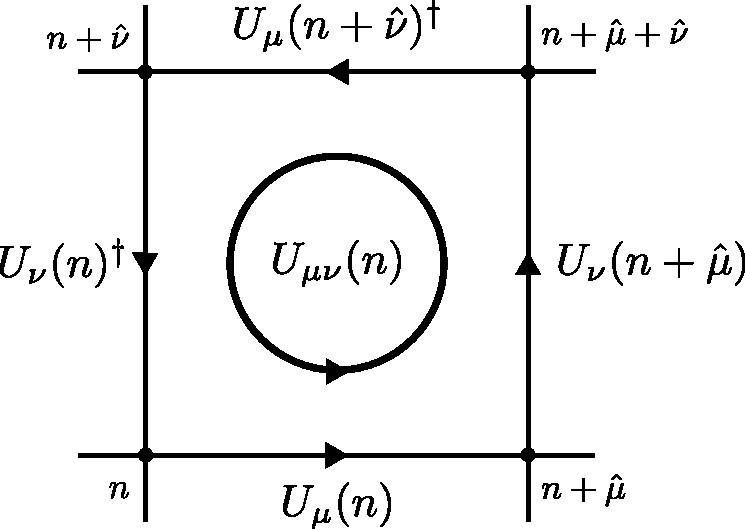
\includegraphics[width=0.5\linewidth]{images/plaquette.pdf}
    \caption{The smallest non-trivial loop on the lattice.}
    \label{fig:plaquette}
\end{figure}
Using this expression we can define a lattice version of the gauge action. To this end we first have to express the plaquette via the continuum variable $A_\mu$ instead of the link variables using equation \eqref{eq:linkVarAndGluonField}. Since the arguments of the exponential functions are matrices we have to use the Baker-Campbell-Hausdorff formula to reduce the product of exponentials to a single exponential. After expanding all gluon fields at the lattice site $n$ to linear order we are left with the approximation
\begin{align}
    U_{\mu\nu}(n)&=\exp\rbr{ia^2(\partial_\mu A_\nu(n)-\partial_\nu A_\mu(n))+i\sqbr{A_\mu(n),A_\nu(n)}+\mathcal O(a^3)}\\
    &=\exp(ia^2G_{\mu\nu}(n)+\mathcal{O}(a^3)).
\end{align}
The lattice gauge is now defined as
\begin{equation}
    S_G[U]=\frac{2}{g^2}\sum_{n\in\Lambda}\sum_{\mu<\nu}\text{Re tr}\sqbr{\mathbb1-U_{\mu\nu}(n)}.
\end{equation}
To see that this expression converges to the continuum action for $a\to0$ we expand the exponential function and use the anti-symmetry of the exponent
\begin{align}
    &\frac{2}{g^2}\sum_{n\in\Lambda}\sum_{\mu<\nu}\text{Re tr}\sqbr{\mathbb1-U_{\mu\nu}(n)}\\
    =&\frac{1}{g^2}\sum_{n\in\Lambda}\sum_{\mu<\nu}\rbr{\text{tr}\sqbr{\mathbb1-U_{\mu\nu}(n)}+\text{tr}\sqbr{\mathbb1-U_{\mu\nu}^\dagger(n)}}\\
    =&\frac{1}{g^2}\sum_{n\in\Lambda}\sum_{\mu<\nu}\rbr{\text{tr}\sqbr{\mathbb1-U_{\mu\nu}(n)}+\text{tr}\sqbr{\mathbb1-U_{\nu\mu}(n)}}\\
    =&\frac{1}{g^2}\sum_{n\in\Lambda}\sum_{\mu,\nu}\text{tr}\sqbr{\mathbb1-U_{\mu\nu}(n)}\\
    =&\frac{1}{g^2}\sum_{n\in\Lambda}\sum_{\mu,\nu}\text{tr}\sqbr{\mathbb1-\mathbb 1 -ia^2G_{\mu\nu}(n)+\frac{a^4}{2}G_{\mu\nu}^2(n)+\mathcal{O}(a^6)}\\
    =&\frac{1}{g^2}\sum_{n\in\Lambda}\sum_{\mu,\nu}\text{tr}\sqbr{-ia^2G_{\mu\nu}(n)}+\text{tr}\sqbr{\frac{a^4}{2}G_{\mu\nu}^2(n)}+\mathcal{O}(a^6)\\
    =&\frac{a^4}{2g^2}\sum_{n\in\Lambda}\sum_{\mu,\nu}\text{tr}\sqbr{G_{\mu\nu}^2(n)}+\mathcal{O}(a^2).
\end{align}
In the limit the sum together with the $a^4$ becomes an integral and the error goes to 0 resulting in the continuum action. Note that $G_{\mu\nu}^2$ is to be understood as squaring the matrix element and we explicitly write the sum over the indices, while in \eqref{eq:qcdLagr} the notation used implicitly summed over the indices\cite{gattringer}.
\todoin{Show that this expression is in the limit the same as the continuum version}

\subsection{Symanzik Improvement: Lüscher-Weisz Gauge Action}
The Wilson Gauge Action goes to the continuum action in the limit. But for finite lattice spacing $a$ the action has an error of order $\mathcal O (a^2)$. The choice of the lattice action is not unique, and there are multiple ways of defining them as long as they converge to the continuum version in the limit. To improve the results of the lattice calculations, it would be favorable to reduce the error. This is the goal of the Symanzik improvement program. The idea is to add more terms and to choose the coefficients in such a way that the leading error is canceled. A typical example is the idea of improving the first order derivative approximation by adding terms that are used to approximate the third derivative. This results in an error that is two orders smaller in $a$.\\
Martin Lüscher and Peter Weisz used this program to improve the Wilson gauge action. Instead of using only all plaquettes on the lattice, they defined the Lüscher-Weisz action by also looking at all (planar) rectangles, parallelograms and bent rectangles, as can be seen in figure \ref{fig:luescherLoops}. In their paper \cite{luscherWeiszAction} they have shown that at tree level we only need to consider the square and rectangular loops to cancel the $\mathcal{O}(a^2)$ error of the Wilson gauge action. The Lüscher-Weisz action is given by
\begin{equation}
    S_{G,LW}=\frac{2}{g^2}\cbr{\frac{5}{3}\sum_\square\text{tr } \sqbr{\mathbb 1-U(\square)}-\frac{1}{12}\sum_\rectangle \text{tr}\sqbr{\mathbb 1-U(\rectangle)}}.
\end{equation}
$U(\square)$ is to be understood as the plaquette defined in equation \eqref{eq:plaquette} and $U(\rectangle)$ is constructed analogously. We sum over all squares but treat squares that differ only in their orientation (e.g. $U_{\mu\nu}$ and $U_{\nu\mu}$) as the same and we do the same for the rectangles.

\begin{figure}
    \centering
    \includegraphics[width=0.5\linewidth]{images/luescherLoops.png}
    \caption{Loops considered in the improved gauge action.}
    \label{fig:luescherLoops}
\end{figure}

\todoin{introduce the idea of tadpole improvement and then introduce the action}

%\subsection{The Haar Measure}
\todoin{still thinking about how much i should mention about it (or if i should mention it at all)}


\section{The Fermionic Part of the Action}
\todoin{Fermions are complicated, and even more on the lattice}

\subsection{Wilson Fermion Action}
Discretizing the fermionic part of the QCD action
\begin{equation}
    S_F =\int d^4x\,\bar\psi(x)\rbr{\slashed D +m}\psi(x) 
\end{equation}
could be done naively by substituting the continuum derivative by the symmetric finite difference quotient and then include link variables to ensure the gauge invariance. This leads to the naive lattice fermion action
\begin{equation}
    S_{\text{F,naive}}=a^4\sum_{n\in\Lambda}\bar\psi(n) \rbr{\gamma_\mu\frac{U_\mu(n)\psi(n+\hat\mu)-U_{-\mu}(n)\psi(n-\hat\mu)}{2a}+m\psi(n)}.
\end{equation}
To see the problem with this formulation we rewrite the expression while stating all indices (except the fermion flavor) explicitly 
\begin{align}
    a^{-4}S_{\text{F,naive}}=\sum_{n,m\in\Lambda}\bar\psi(n)_{a\alpha} D(n|m)_{ab\alpha\beta}\psi(m)_{b\beta}
\end{align}
with
\begin{equation}
    D(n|m)_{ab\alpha\beta}=\rbr{\gamma_\mu}_{\alpha\beta}\frac{U_\mu(n)_{ab}\delta_{n+\hat\mu,m}-U_{-\mu}(n)_{ab}\delta_{n-\hat\mu,m}}{2a}+m\delta_{nm}\delta_{ab}\delta_{\alpha\beta}.
\end{equation}
Following the derivation in \cite{gattringer} we can compute the Fourier transform of $D(n|m)$ for the case of setting all link variables to unity
\begin{align}
    \tilde{D}(p|q)&=\frac{1}{\lvert\Lambda\rvert}\sum_{n,m\in\Lambda}e^{-ipna}D(n|m)e^{iqma}\\
    &=\delta(p-q)\rbr{m\mathbb 1 +\frac{i}{a}\sum_\mu\gamma_\mu\sin(p_\mu a)}\\
    &=\delta(p-q)\tilde D(p).
\end{align}
For $m=0$ the inverse is given by
\begin{equation}
    \tilde D(p)^{-1}=-ia\frac{\sum_\mu\gamma_\mu\sin(p_\mu a)}{\sum_\mu\sin(p_\mu a)^2}.
\end{equation}
This is the propagator whose poles describe particles. In the continuum limit $a\to0$ the only pole is for $p=0$. For non-zero $a$ however, we get a pole when $\sin(p_\nu a)$ is zero for all $\nu$. On the lattice the momentum range in every direction is $(-\pi/2,\pi/2]$, giving rise to 16 poles. These lattice artifacts are called fermion doublers, since we have 16 fermions for every single physical fermion\cite{gattringer}. 

\todoin{write the naive version by substituting the continuum derivative by its lattice counterpart.}
\todoin{Link variables and their transformation}
\todoin{maybe the connection the link variables and the field via gauge transporter}

\subsection{Wilson Fermion Action}
To remove these doublers Wilson introduced an additive term, the Wilson term, so that the Fourier transform becomes
\begin{equation}
    \tilde D(p)=m\mathbb1+\frac{i}{a}\sum_\mu\gamma_\mu\sin(p_\mu a)+\mathbb1\frac{1}{a}\sum_\mu\rbr{1-\cos(p_\mu a)}.
\end{equation}
This extra term vanishes for $p=0$ while it adds the term $\frac2a$ for each momentum component taking the value $\frac{\pi}{a}$ which can be thought of as an additional mass term. In the continuum limit this new mass diverges and these extra poles decouple from the theory leaving us with a single fermion\cite{gattringer}.

\todoin{Fermion doubling problem and its solution with the extra term}
\subsection{Chiral symmetry and the Nielsen-Ninomiya theorem}
The QCD Lagrangian satisfies the chiral symmetry in the massless case, which is also the reason why we call this case the chiral limit. In the continuum this symmetry implies that the Lagrangian does not change when we rotate the spinor fields according to
\begin{equation}
    \psi^\prime=\exp(i\alpha\gamma_5)\psi,\qquad \bar\psi^\prime=\bar\psi\exp(i\alpha\gamma_5)
\end{equation}
introducing the fifth gamma matrix
\begin{equation}
    \gamma_5:=\gamma_1\gamma_2\gamma_3\gamma_4
\end{equation}
which anticommutes with the other gamma matrices
\begin{equation}
    \cbr{\gamma_5,\gamma_\nu }=0.
\end{equation}
Using this property, it follows that in the chiral limit the symmetry is fulfilled. This symmetry and its spontaneous breaking explain important mass related properties in QCD and cannot be simply ignored.\\
On the lattice we loose the chiral symmetry in Wilson's formulation even in the massless case. The reason for this is that the Wilson term behaves like a mass term and thus breaks the symmetry exactly like the mass term outside the chiral limit.\\
The Nilesen-Ninomiya theorem destroys the hope that by choosing another way of discretizing the theory, we may overcome this problem. It states that on the lattice we cannot ensure chiral symmetry and remove the fermion doublers at the same time. \\
One way of solving this problem is to define a lattice version of the chiral symmetry that goes into the continuum version for $a\to 0$. Another approach that has other problems but is computationally faster is the staggered fermion formulation\cite{gattringer}.


\subsection{(Highly Improved) Staggered Quark action}
\todoin{I am still thinking about this}

In the staggered fermions formulation, which are also called Kogut-Susskind fermions, we keep the continuum chiral symmetry while reducing the number of fermion doublers from 16 to four. The idea is to transform the spinor field so that the Dirac operator is diagonal in spinor space so that we can discard all but one component. \\
We start by performing a position dependent rotation of the Dirac spinors in the spinor space
\begin{equation}
    \psi(n)=\gamma_1^{n_1}\gamma_2^{n_2}\gamma_3^{n_3}\gamma_4^{n_4}\psi(n)',\quad \bar\psi(n)=\bar\psi(n)'\gamma_4^{n_4}\gamma_3^{n_3}\gamma_2^{n_2}\gamma_1^{n_1}
\end{equation}
with
\begin{equation}
    n=(n_1,n_2,n_3,n_4).
\end{equation}
Since the square of each gamma matrix is just the identity, it follows that the mass term is invariant under this rotation. The derivative term transforms non-trivially since it contains gamma matrices and compares fields at different lattice sites. Using the Clifford algebra we find
\begin{align}
    \bar\psi(n)\gamma_1\psi(n\pm\hat1)&=\bar\psi(n)'\mathbb1\psi(n\pm\hat1)'\\
    \bar\psi(n)\gamma_2\psi(n\pm\hat2)&=\bar\psi(n)'\mathbb1\psi(n\pm\hat2)'(-1)^{n_1}\\
    \bar\psi(n)\gamma_3\psi(n\pm\hat3)&=\bar\psi(n)'\mathbb1\psi(n\pm\hat3)'(-1)^{n_1+n_2}\\
    \bar\psi(n)\gamma_4\psi(n\pm\hat4)&=\bar\psi(n)'\mathbb1\psi(n\pm\hat4)'(-1)^{n_1+n_2+n_3}
\end{align}
with $\hat i$ denoting one step in the $i$ direction. Introducing the staggered sign function $\eta_\mu(n)$ we may summarize the previous equations via
\begin{equation}
    \bar\psi(n)\gamma_\mu\psi(n\pm\hat\mu)=\eta_\mu(n)\bar\psi(n)\psi(n\pm\hat\mu).
\end{equation}
The naive fermion Lagrangian expressed in the transformed fields reads
\begin{equation}
    \lagr(\psi, \bar\psi)=\bar\psi(n)'\mathbb1\rbr{\sum_\mu\eta_\mu(n)\frac{\psi(n+\hat\mu)'-\psi(n-\hat\mu)'}{2a}+m\psi(n)'}.
\end{equation}
The Dirac operator is now diagonal in the spinor space. Thus, we may keep only one component and receive the staggered fermion action 
\begin{equation}
    S_F[\chi,\bar\chi]=a^4\sum_{n\in\Lambda}\bar\chi(n)\rbr{\sum_\mu\frac{U_\mu(n)\chi(n+\hat\mu)-U_{-\mu}(n)\chi(n-\hat\mu)}{2a}+m\chi(n)}.
\end{equation}
To see that the action satisfies the chiral symmetry (in the chiral limit), we first need to find the corresponding chiral transformation for the transformed fields. Using once again the commutation relations of the gamma matrices, we find
\begin{equation}
    \bar\psi(n)\gamma_5\psi(n)=(-1)^{n_1+n_2+n_3+n_4}\bar\psi(n)'\psi(n)'=:\eta_5(n)\bar\psi(n)'\psi(n)'.
\end{equation}
In the chiral limit this means that our new fields transform via
\begin{equation}
    \chi(n)'=\exp(i\alpha\eta_5(n))\chi(n),\quad\bar\chi(n)'=\exp(i\alpha\eta_5(n))\bar\chi(n)
\end{equation}
and the chiral symmetry follows as can be seen from
\begin{align}
    &\bar\chi(n)'\chi(n\pm\hat\mu)'\\
    =&\bar\chi(n)'e^{i\alpha\eta_5(n)}e^{i\alpha\eta_5(n\pm\hat\mu)}\chi(n\pm\hat\mu)'\\
    =&\bar\chi(n)\chi(n\pm\hat\mu)\exp\sqbr{i\alpha\rbr{(-1)^{n_1+n_2+n_3+n_4}+(-1)^{n_1+n_2+n_3+n_4\pm1}}}\\
    =&\bar\chi(n)\chi(n\pm\hat\mu).
\end{align}
Since the staggered fermions are Grassmann variables we may use the same trick to write the integral over the fermions fields as the fermion determinant. Since we still have four fermions for each physical fermion, which are called tastes, it is common practice to take the fourth root of the determinant.\\
In our simulations we will not use the staggered fermion action, but the Highly Improved Staggered Quark (HISQ) action\cite{hisq}. This improved action eliminates tree level errors resulting from taste exchange interactions by smearing the link variables and finite difference errors of order $\mathcal O(a^2)$ by including further terms.\cite{bielefeldPHD}